% !TEX encoding = UTF-8 Unicode
% -*- coding: UTF-8; -*-
% vim: set fenc=utf-8

\chapter{Arquitetura ARMFUL}%
\label{chap:arquitetura-armful}

Nesse capítulo será apresentada a arquitetura \abbrev{ARMFUL}{Analysis of Raw Data from Multiple Files} ARMFUL (do inglês: Analysis of Raw Data from Multiple Files; em tradução livre: Análise de Dados Científicos de Múltiplos Arquivos), introduzida recentemente em~\cite{silva2016situ,silva2017raw} pelo laboratório de \abbrev{NACAD}{Núcleo Avançado de Computação de Alto Desempenho} Núcleo Avançado de Computação de Alto Desempenho (NACAD) da \abbrev{UFRJ}{Universidade Federal do Rio de Janeiro} UFRJ (Universidade Federal do Rio de Janeiro). Também será abordado o \textit{DfAnalyzer}, uma instância dessa arquitetura, implementada pelo mesmo laboratório.

\section{Visão geral}

A \textbf{arquitetura ARMFUL} tem suporte a extração de dados científicos, a técnicas de indexação e a análise de dados científicos a partir de múltiplos arquivos~\cite{silva2016situ} com o propósito de permitir o acesso direto a qualquer elemento ou região específica do espaço do fluxo de dados de uma simulação científica. Essa flexibilidade na análise existe graças a uma \textbf{arquitetura de componentes}, que utiliza um SGWfC como bancos de dados de proveniência de dados para proporcionar um caminho de acesso entre o fluxo de dados e os dados científicos~\cite{silva2017raw}.

% Baseado na seção 5 de~\cite{silva2017raw}. Tentativa de tradução livre e de adaptação para o contexto desse trabalho.
A ARMFUL funciona do seguinte modo: a gerência de conteúdos científicos é obtida a partir de dados científicos de arquivos, que então são relacionados, em um SGBD relacional, através de dados de proveniência do fluxo de dados. Essa gerência de dados requer características que são específicas do domínio; por isso, modelos de dados de proveniência costumam ser representados em granularidade não-fina. Entretanto, consultas de proveniência possuem um valor analítico limitado caso não sejam relacionadas a elementos de dados específicos ao domínio da simulação científica. Só que isso exige bastante esforço de usuários de SGWfC no que diz respeito a desenvolver, para cada domínio, um modelo de dados e programas científicos específicos para acessar, extrair e relacionar os dados de domínio aos dados de proveniência. Nesse aspecto, a arquitetura ARMFUL contribui objetivando a colaborar com esse esforço através da introdução e apresentação de componentes genéricos que modelam e relacionam entre si, no mesmo banco de dados, dados específicos de domínio e proveniência.

\perrotta{TODO: extraction cartridge}
\perrotta{TODO: relational DMBS}

Na \autoref{fig:armful-architecture}, podemos visualizar como é feita a divisão em componentes da ARMFUL, que são os seguintes:

\begin{itemize}
    \item Extração de dados científicos;
    \item Indexação de dados científicos;
    \item Catálogo de dados científicos;
    \item Ingestão de dados de proveniência;
    \item Processamento de consultas.
\end{itemize}

\begin{figure}[ht]
    \centering
    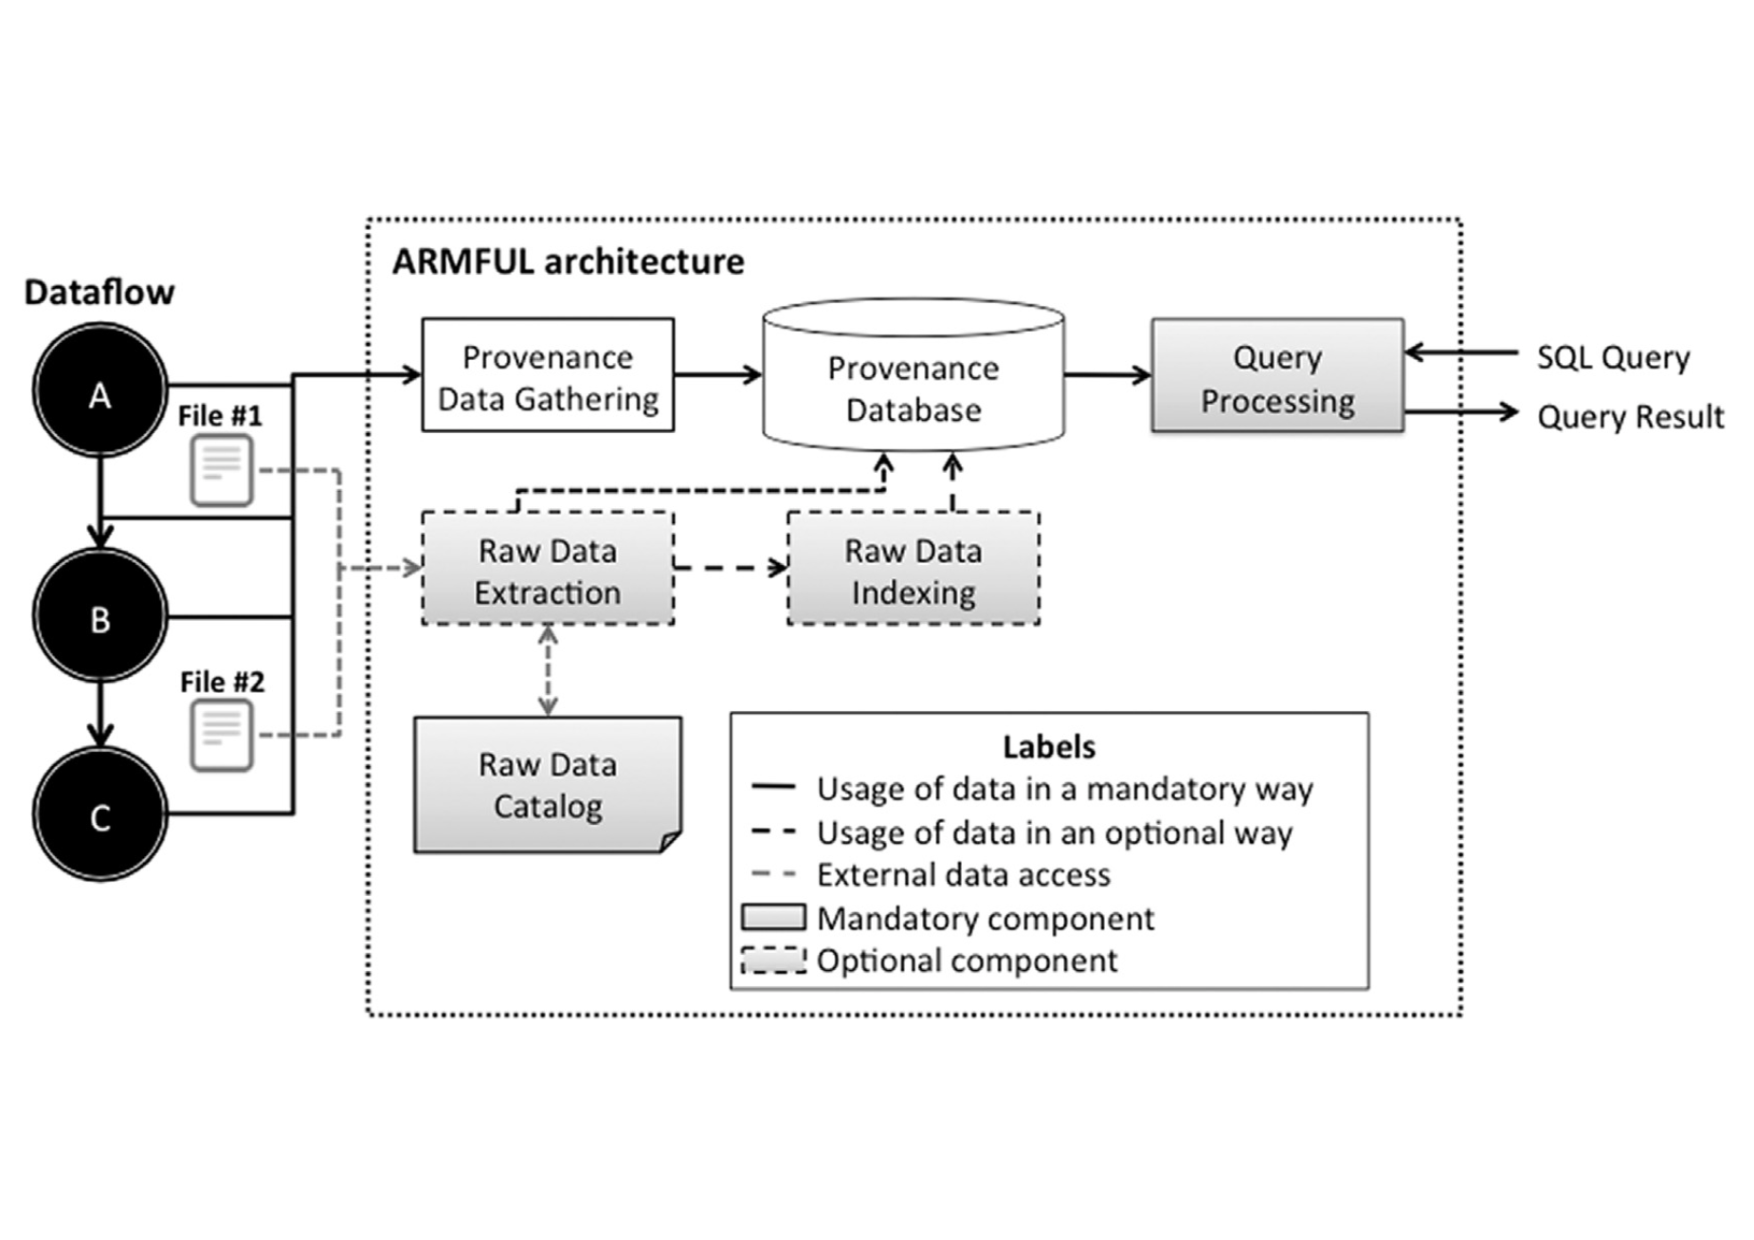
\includegraphics[width=\textwidth]{img/armful-architecture}
    \caption[Componentes da arquitetura ARMFUL]{Componentes da arquitetura ARMFUL. Encontrada originalmente em~\cite{silva2017raw}.}%
    \label{fig:armful-architecture}
\end{figure}

Os componentes na cor branca correspondem à captura e ao armazenamento de dados de proveniência em um banco de dados de proveniência. Em contrapartida, os componentes na cor cinza descrevem os passos responsáveis por: (\(i\)) extrair dados científicos de arquivos, (\(ii\)) gerar índices para os mesmos e (\(iii\)) permitir a consulta de proveniência \textbf{e} dados científicos a partir do mesmo banco de dados. Nas próximas subseções, os componentes serão detalhados.

% Baseado na seção 5.1 de~\cite{silva2017raw}.
\subsection{Extração e indexação de dados científicos}

O \textbf{componente de extração de dados científicos} tem o objetivo de ler o conteúdo de arquivos científicos, analisá-lo e então recuperar parte do conteúdo selecionado que é relevante de acordo com os atributos especificados pelo usuário. Para que esse objetivo seja completado, quatro etapas devem ser seguidas:

\begin{itemize}
    \item \textbf{leitura do conteúdo}: acesso aos arquivos científicos e leitura do seu conteúdo;
    \item \textbf{tokenização}: investigação do catálogo de dados científicos, que contém metadados relacionados à especificação do formato de arquivo, visando verificar se os dados científicos obtidos na etapa anterior correspondem ao domínio da simulação computacional processada atualmente;
    \item \textbf{filtragem de conteúdo}: a especificação do usuário é responsável por definir e restringir o que deve ser analisado e armazenado no banco de dados de proveniência, isto é, essa etapa evita armazenar atributos desnecessários, que não serão utilizados na próxima etapa;
    \item \textbf{análise}: conversão de ada dado científico filtrado em uma estrutura de dados adequada para ser armazenada no SGBD. Os requisitos dessa estruturas de dados são documentados no catálogo de dados científicos.
\end{itemize}

O \textbf{componente de indexação de dados científicos} visa indexar um conteúdo específico dos arquivos científicos a fim de melhorar o tempo e desempenho de acesso direto a determinadas regiões do espaço de dados científicos através da gerência de metadados correlacionados ao fluxo de dados. A criação de índices é realizada segundo um algoritmo de indexação previamente definido.

\perrotta{REVIEW: Mencionar exemplos de bitmap indexing e positional index??}

% \subsection{Catálogo de dados científicos}

\subsection{Ingestão de dados}

% prov df (alimentar a base de dados com informacoes de proveniencia)
% ProvenanceGatherer

\subsection{Processamento de consultas}

% QueryProcessor

% melhor traduzir tudo, exceto DfAnalyzer

\section{DfAnalyzer: uma instanciação da arquitetura ARMFUL}

% DfAnalyzer (instância da ARMFUL) --> conjunto de componentes
% Provenance Gatherer (origem da proveniência para o banco de dados que eu vou utilizar na QueryProcessor)
% QueryProcessorCaptura de dados de proveniência}

\subsection{Provenance Data Gatherer (PDG)}

\subsection{Raw Data Extractor (RDE)}

\subsection{Raw Data Indexer (RDI)}

% \subsection{Catálogo de dados científicos?}

\subsection{Query Processor (QP)}